\makeatletter
\begin{figure}[H]
\centering
\resizebox{.8\textwidth}{!}{%
    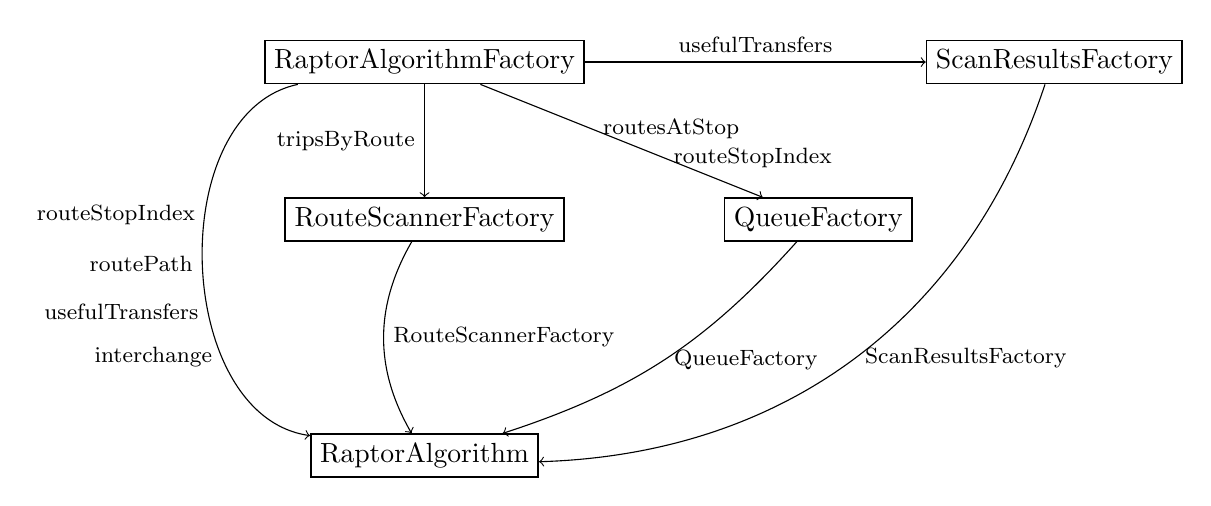
\begin{tikzpicture}[rect/.style={shape=rectangle,draw=black,semithick,align=center},
    ]
    % QueueFactory(, ),
    %       new RouteScannerFactory(tripsByRoute),

        
    % draw nodes
    \node[rect] (RaptorAlgorithmFactory) at (2,0) {RaptorAlgorithmFactory};
    \node[rect] (ScanResultsFactory) at (10,0) {ScanResultsFactory};
    \node[rect] (QueueFactory) at (7,-2) {QueueFactory};
    \node[rect] (RouteScannerFactory) at (2,-2) {RouteScannerFactory};

    \node[rect] (RaptorAlgorithm) at (2,-5) {RaptorAlgorithm};
    
    \draw (RaptorAlgorithmFactory) edge[->] node[above,pos=0.5,font=\footnotesize] {usefulTransfers} (ScanResultsFactory);

    \draw (RaptorAlgorithmFactory) edge[->] node[right,pos=0.4,font=\footnotesize] {routesAtStop} node[right,pos=0.65,font=\footnotesize] {routeStopIndex} (QueueFactory);

    \draw (RaptorAlgorithmFactory) edge[->] node[left,pos=0.5,font=\footnotesize] {tripsByRoute} (RouteScannerFactory);

    \draw (RaptorAlgorithmFactory) edge[->, bend right=80] node[left,pos=0.4,font=\footnotesize] {routeStopIndex} node[left,pos=0.5,font=\footnotesize] {routePath} node[left,pos=0.6,font=\footnotesize] {usefulTransfers} node[left,pos=0.7,font=\footnotesize] {interchange} (RaptorAlgorithm);
    
    \draw (RouteScannerFactory) edge[->,bend right=30] node[right,pos=0.5,font=\footnotesize] {RouteScannerFactory} (RaptorAlgorithm);

    \draw (QueueFactory) edge[->, bend left=15] node[right,pos=0.5,font=\footnotesize] {QueueFactory} (RaptorAlgorithm);

    \draw (ScanResultsFactory) edge[->,bend left=35] node[right,pos=0.5,font=\footnotesize] {ScanResultsFactory} (RaptorAlgorithm);
    
    \end{tikzpicture}
    }
    \caption{This represents the dataflow of the \glsxtrshort{raptor} in order to createan RaptorAlgorithm}
    \label{fig:dataflow}
\end{figure}
\makeatother